\documentclass[10pt,twocolumn]{article} 

\usepackage{oxycomps} % use the main oxycomps style file
\usepackage{amsmath}

\usepackage{array, booktabs, longtable}
\usepackage{graphicx}
\usepackage[x11names, table]{xcolor}
\usepackage{caption}
\DeclareCaptionFont{blue}{\color{LightSteelBlue3}}

\newcommand{\foo}{\color{LightSteelBlue3}\makebox[0pt]{\tiny\textbullet}\hskip-0.5pt\vrule width 1pt\hspace{\labelsep}}
\newcommand{\bfoo}{\raisebox{2.1ex}[0pt]{\makebox[\dimexpr2\tabcolsep]%
{\color{LightSteelBlue3}\tiny\textbullet}}}%
\newcommand{\tfoo}{\makebox[\dimexpr2\tabcolsep]%
{\color{LightSteelBlue3}$\boldsymbol \uparrow $}}%

\bibliography{references}

\pdfinfo{
    /Title (AI-Chinese Chess)
    /Author (Haotian wang)
}

\title{AI-Chinese Chess}

\author{Haotian wang}
\affiliation{Occidental College}
\email{hwang2@oxy.edu}

\begin{document}

\maketitle

\section{Problem Context}
    Xiangqi, also known as the elephant chess or the Chinese chess game, is a strategy board game for two players. It is one of the most popular board games in China. Chinese chess uses a square checkered board with 32 round pieces, 16 in each of the two colors red and black, placed and moving at intersections. The first player to "checkmate" the opponent's general wins. Just like any other chess or board games, Xianqi consist a great deal of combination moves and strategies\cite{XiangQi}.
    People used to practice and play Xiangqi in the real world with either friends or arranged competitors in competitions. However, due to. the outbreak of Covid-19 pandemic, chess players often needs to be quarantined due to varies reasons, especially in China, where the lock down policies are extremely strict. Many of the competitions and practice arrangements are cancelled. Players are forced to either play online and practices online.  Players often have few options to choose who they can play to and where they can practice their skills. 
    
    AI and machine learn has been widely successful in applications for all kind of purposes in almost every field of work. In context, AI and machine learn has been solutions for various kind of strategy or decision making programs. AI is also used to test out human limits. The main advantage of using AI models to make decisions and plan strategies is that the the algorithms and computing power can provide the client the most accurate or best suited strategy with minimal bias factors in short time. Even though there are various kind of AI model for the Xiangqi already. However, the access for these projects are limited to very few player. Players are not able to access these AI models to train themselves. In addition, these models are generally made to test algorithms and compete with other AI models\cite{4M}. Since most AI models are used to test the limitations of the algorithms, the level of difficulty increases as well. General players who didn't reach that level will only defeat without knowing how to improve. 
    
\section{Technical Background}
	This implementation will require knowledge of reinforced deep learning, neural network, 
	Monte Carlo tree search, programming language and HTML. This implementation uses reinforcement learning based on deep neural network training. It adopts a self play learning model constructed by combining deep convolutional neural networks and Monte Carlo search tree algorithm, and uses MCTS algorithm to simulate chess moves that constantly change roles. 
	
	The deep convolutional neural network inputs mainly the current chessboard state and then outputs the likelihood of each move and the current player's victory rate via the deep convolutional neural network.\cite{MCTSAG} If the deep convolutional neural network is \(f\), the deep neural network can be stated as follows:
	\[(p,v)=f_\theta(s)\]
	
	In addition,\(s\) represents the current state of the chessboard, \(p\) represents the likelihood of each move, and $p_a = Pr (a|s)$ represents the probability of each move. The current player's victory percentage is denoted by \(v\). The MCTS tree algorithm partially relies on the output results of \(f\) to direct MCTS to perform multiple simulation moves from the root node to the leaf node, so it can select a better winning rate strategy. Assume the MCST algorithm is \(\varphi_\theta\), then the MCST algorithm can be as follow:
	\[(\pi,z)=\varphi_\theta(p,v,N,Q)\]\cite{EMCTSXQ}
	
	In this context, \(\pi\) represents the probability of each move output by the final reinforcement learning model, and \(z\) is the winning rate of the player who makes the first move in the game.\cite{Wenzhi} The input of the MCST algorithm is the output \((p,v)\) of \(f_\theta\) combined with the number of visits \(N\) and the average action value \(Q\) in each iteration. When a game of chess is finished, the neural network's training goal is to maximize the similarity between $(p, v)$ and $(\pi, z)$, and then continually increase the neural network's processing power in self-learning.
	
	For each position the player moves, the algorithm use the latest deep neural network result to guide the MCTS to search for the move probability of each position. Each position consist \(I\) legal moves, then the move probability represents for the move corresponds to the probability of the move. The appropriate move is chosen for each position. Based on the above pattern, the until the game reaches the one player winning situation or check mate, the winner Z will be the next output. After the winner occurs, the neural network will be trained in the reverse direction according to the winner.
	
	\begin{figure}
        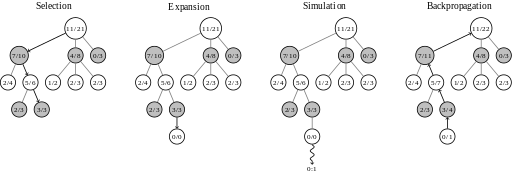
\includegraphics[width=\linewidth]{MCTS.png}
        \caption{MCTS}
        \label{fig1:Monte Carlo Tree search}
    \end{figure}
	
	Selection is the first stage in a Monte Carlo tree search. Begin with the root R and progress through the child nodes until you reach the leaf node L. The current game state is represented by the root, and a leaf is any node with a potential child but no simulation (play out) has yet been initiated. The section that follows goes into greater detail on a method of biasing the selection of child nodes that allows the game tree to expand towards the most promising moves, which is the essence of Monte Carlo tree search. Unless L finishes the game decisively (e.g., win/loss/draw) for either player, the second stage is expansion.\cite{Report} Create one (or more) offspring nodes and select node C from one of them. Any legitimate move from the game position described by L is a child node. The third stage is simulation, which is accomplished by completing one random play out from node C. This process is also known as play out or roll out. A play out could be as easy as selecting uniform random moves till the game is over (for example in chess, the game is won, lost, or drawn). Back propagation is the final stage, which uses the results of the play out to update information in the nodes on the path from C to R.
	
	
\section{Prior Work}
    Artificial Inteligence and Machine learning algorithm models are one of the most widely employed methods for decision and strategy projects. In this section we will focus on the prior works done in using AI and ML models implemented in other strategy games, especially the Monte Carlo tree search implementation, as it is the one of the most important part of this project 
\subsection{Alpha Go Zero}
    The game "Go" is played with a rectangular board and black and white circular pieces. There are 19 lines and 361 intersections on the regular board, and the pieces must move on the intersections where spaces are not forbidden. Because Black has a first move advantage, Black is artificially required to give White an eye at the end of the game. AlphaGo Zero is a computer software that combines a deep neural network with an advanced search tree. As an input, these neural networks process a description of the Go board through a number of network layers comprising millions of neuron-like connections. The "policy network," a neural network, chooses the next move to play. The "value network," the other neural network, predicts the game's winner. We exposed AlphaGo Zero to a variety of amateur games in order to help it build a grasp of reasonable human play. Then we let it play thousands of times against different versions of itself, each time learning from its mistakes. AlphaGo Zero evolved over time, becoming ever stronger and better at learning and decision-making. This is referred to as reinforcement learning. AlphaGo Zero went on to defeat Go world champions in many worldwide arenas, establishing himself as the greatest Go player of all time.In a Go game, AlphaGo Zero builds a local policy to sample the next move using MC Tree Search. MCTS looks for potential moves and stores the results in a search tree. As more searches are made, the tree and its information grow in size. \cite{Surag}
    
    

\subsection{Deep blue}
    Deep Blue was a chess-playing expert system that ran on a one-of-a-kind IBM supercomputer. It was the first computer to win a game and the first to win a match against a defending world champion in regular time.
    Deep Blue's evaluation function was first developed in a generalized manner, with many parameters still to be defined. Thousands of master games were analyzed to get the values for these factors. The evaluation function was then divided into 8,000 pieces, many of which were intended for specific roles. The opening book featured almost 4,000 positions and 700,000 grand master games, while the endgame database included many six-piece endgames as well as all five and fewer piece endgames. An supplementary database known as the "extended book" summarizes whole grand master games. To identify opening moves, the algorithm combines its ability to search 200 million chess positions per second with summary information from the extended book. \cite{DeepBlue}
    \begin{figure}
        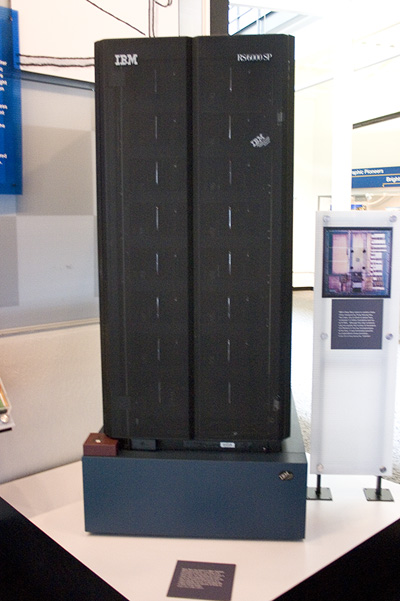
\includegraphics[width=90]{Deep_Blue.jpg}
        \caption{Deep Blue cabinets}
        \label{fig2:Deep Blue}
    \end{figure}
    
\section{Methodology}
    For this AI-Chinese chess project, i propose to Machine learning, specifically Reinforcement learning and the Monte Carlo Tree search algorithm. In addition, This project will be hosted online using HTML.
    
\subsection{Language and platform}
    In this project, i propose to use Python for the this project. The benefits includes simplicity and consistency, access to great libraries and frameworks for AI and Chine leaning, flexibly and platform independence.
    
\subsection{Machine and platform}
    For the Machine and platform that I will use to do the self play, train, and evaluation process will be done on the occidental cluster computer for the convenience of its computing power. This will largely decrease my training time. 

\subsection{Feature extractor, Policy network and Value net work}
    The who project is made up of three interconnected neural networks: a feature extractor, a policy network, and a value network. This is also why AlphaGo Zero is sometimes referred to as the two-headed beast: it has a body (the feature extractor) and two heads (policy and value). The feature extractor model generates its own board state representation. The policy model generates a probability distribution across all possible moves, while the value model generates a scalar value in the range [1;1] to signify which player is more likely to win based on the current condition of the board. The output of the feature extractor is used as input by both the policy and value models.\cite{Java}

\subsection{Monte Carlo tree search}
    \begin{itemize}
    \item Each node in the tree represents a board state and stores various statistics, including the number of times the node has been visited (n), the total action value (w), the prior probability of reaching that node (p), the mean action value (q, which is q=w/n), the move made from the parent to reach that node, a pointer to the parent node, and finally all the legal moves from this node that have a non-zero probability as children\cite{Java}.
    \item During the initial phase, the algorithm starts with a root node and chooses a child node with the highest win rate. We also want to ensure that each node has an equal probability. The goal is to keep selecting optimum child nodes until we reach the tree's leaf node. UCT is a nice approach to find such a child node\cite{Java}.
    \item Expansion: When it is unable to discover the successor node using UCT, it grows the game tree by adding all potential states from the leaf node.
    \item Following Expansion, the algorithm selects a child node at random and simulates a randomized game from the selected node until it reaches the game's resulting state. Light play out occurs when nodes are chosen at random or semi-randomly throughout the play out. You can also choose to put in a lot of effort by writing quality heuristics or evaluation functions\cite{Java}.
    \item When the algorithm approaches the end of the game, it evaluates the state to determine which player has won. It traverses upwards to the root and increases the visit score for all visited nodes. It also updates the win score for each node if the player for that position wins the play out. MCTS maintains repeating these four phases until a set number of iterations or a fixed length of time has passed. Based on random motions, we estimate the winning score for each node in this method. The greater the number of iterations, the more reliable the estimate gets. The algorithm estimations will be less accurate at the start of a search and will continue to improve after a significant length of time. Again, it is totally dependent on the nature of the problem.\cite{Dylan}
\subsection{Self-play}
    The self-play component is in charge of data generation. It works by having the best agent in the world play against itself. When a game ends (either by the two players passing, one of the players resigning, or the number of moves exceeding a certain threshold), every registered action of the game is updated with the game's winner, changing the shape from (board state, move, player color) to (board state, move, winner). Every time a batch is formed, the process checks to see if the current agent being used to generate games is still the best agent. The following function is a rough sketch of how self-play works in practice.\cite{Dylan}

\subsection{Training}
    In addition, the training is relatively simple. Using the newly generated games, the existing best agent is taught. To enhance the size of the data set, each state in the data set is increased by applying all of the dihedral rotations of a square (rotations and symmetries) to it. The training process checks the database every few iterations to see whether the self-play process has generated new games, and if so, the training process retrieves them and changes the data set accordingly. After a few iterations, the trained agent is submitted to asynchronous evaluation in another process. \cite{Dylan}

\subsection{Evaluation}
    The current best agent is pitted against the trained agent using the competitive parameter in the evaluation. They play a given number of games against each other, and if the trained agent wins more than a specific percentage of the time, the trained agent is rescued and becomes the new best agent.\cite{Dylan}

\end{itemize}

\section{Evaluation}
    For This project's evaluation process, I purpose that it should be evaluated in the following three methods and standards: Winning rate; Real human competition feedback; Comparison of Performance in other implementation of Monte Carlo in Chess and Shogi.
\subsection{Winning rate}
    This section of evaluation will be based on three separate winning rate in this project, including the winning rate of each move and each game, along with the winning rate curve through out the game. Here, we use the winning percentage observed in game records instead of the "true" probability estimated by Monte Carlo Simulation by comparing it with the "true probability\cite{}. The significance of this procedure is to verify the reliability of each move's calculation. 
\subsection{Real Human competition feedback}
    During this process of the evaluation, i will invite around 5-10 people and each play 10 games with the AI to test out the gaming ability of the AI. In addition, i will ask players to provide a feedback survey based on the experience, difficulty, and improvements of the AI. This is essential, because the program is design to assist people to train themselves. Thus, user experience is extremely important. 
    
\subsection{Comparison of Performance in other implementation of Monte Carlo implementation}
    In this last process of evaluation, i propose to compare the performance outcome based on accuracy, precision, F-score, win rate and performance time with Alpha Go, and other Monte Carlo implementations on chess and Shigo. The meaning of this process is to evaluate whether  this project successes in matching other projects performance or not. As well as to find weak spots to improve\cite{Accuracy}
\begin{itemize}
    \item is the level of difficulty to hard or too easy for the player; 
    \item is the model performing without mistakes;
\end{itemize}
    
\section{Ethical Consideration}
    The world is almost driven by technologies today, countless innovative products are being invented and introduced to people every day. When the project is designed with ethical and moral standards, it is essential to prevent unequal, unethical, injustice, and harmful events from happening. During the early stages of computer technology, ethical concerns about computers were virtually non-existent because computers were not nearly as complex as they are now. However, ethical circumstances about computers and cyber technology are unavoidable in contemporary civilization. Computer technology permeates every area of our daily life. Different computer technology offers distinct capabilities that enable people to carry out daily tasks effectively and quickly. In recent decades, computer scientists have been trying to produce multiple machine learning AI in chess games and other competitive sports in favor of testing the limitations of both humans and machines. We now live in a world dominated by capitalism and advanced technology. With the more advanced science and technologies, humans tend to apply these techs in various fields to save cost or provide convenience. However, while technologies such as AI is being implemented in different areas, different ethical consideration must be considered and create precautions for it. This paper will examine ethical issues, including power, accessibility, resource consumption, upkeep, and maintenance.
\subsection{General Ethical consideration}
    The general ethical discussion going on for years is should AI exist? Scientists and the general public have discussed this controversial topic for decades. Simple AI and machine learning can provide people convenience in daily life, such as making a living easier using AI-controlled intelligent home devices. More complicated AI may be applied to auto-driving cars or search engines to provide more accurate search results. Scientists even pushed the limitation of AI into making decisions for humans. For instance, A corporate institution may use AI to help them select the employees they need. A college may use AI to filter out those students who aren't qualified for their standards. A court may use AI to judge human crimes based on laws. These examples demonstrate that with the advancement of AI technology to this day, it can replace humans in many positions while providing more efficiency to work. Machines, robots, and algorithms are slowly replacing some people's positions in modern society. The creators and users of AI must set ethical and moral standards for these technologies if the AI trend is unstoppable\cite{EthicalIssue}. It is clear that ethics are not only vital but also critical in reshaping these powerful algorithms in favor of humanity. Machines learn ethics through the programming that is programmed into them. As a result, the creators of these so-called AI algorithms should not take this lightly. Where we are today is the result of millions of years of evolution. When compared to the development of AI fields, we are not nearly a century old since the first computer was invented. The internet is only three decades old. So you can picture the rate of change in the world of artificial intelligence. Without ethics, a field as fast-paced as this would spell tragedy if it fell into the wrong hands\cite{BillGates}.
    
\subsection{Power Consideration}
    There is a potential power ethic issue in the project of training an AI to learn and mimic the human mindset in playing chess. The power issue strands for providing some or a group of people unequal power over others. As a project part of the trend of AI and machine learning, this project potentially acts as a small part of the grand scheme. While the ability of AI can beat the best of humans in other board games, such as Alpha GO winning Lee Sedol in the 'GO' game during the 2016 march, it inspired others to do the same in other chess or board games\cite{AlphaGo}. Even real sports as everyone knows that chess board games and any other sports games are supposed to be fair to play. In the context of this paper, the Chinese chess game should be assumed to be honest and unbiased. With the pandemic happening, more and more people choose to play the Chinese chess game online and compete with other players. A small group of people uses AI to help them win higher-rank games, resulting in a series of unfair games. Evidently, YouTube held dozens of video tutorials on using Online AI to cheat in online chess games. This potentially distributes power to those who use AI in online competitions, Which could be defined as cheating. Moreover, the player playing against those cheaters may have no idea about that, resulting in a bad mood and even doubting their abilities in playing the game. The charming part of a competitive game is about both winning and losing. If someone is only there to experience loss, it may cause them to quit the game forever. This type of cheating is unethical and unacceptable and wholly abandoned the common sense of maintaining a fair competition game environment. The purpose of creating this AI Chinese chess project is to help train players' chess skills while practicing it. Using this project to cheat in online competition games should not be tolerated, yet there are only a few ways to prevent this from happening. The solution found is limited but could potentially be helpful. 

\subsection{Environmental consideration}
    While AI is learning how the human brain functions and uses it to either assist people in work, life, or provide entertainment, these AI's consume tons of energy resources to train the model and cause environmental concerns. For instance, on 45 terabytes of data, OpenAI trained its GPT-3 model. According to the US Energy Information Administration, the average household uses 10,649 kWh per year. As a result, training the final version of MegatronLM consumed nearly the same amount of energy as three homes use in a year\cite{EnergyConsumption}. The heavier the data set is used to train, the more energy and resources it consumes. As the trend of AI rises, a great deal of AI models has been developed and trained in recent decades. Even though these AI models may contribute to society, individuals, or organizations in certain ways, the creator must not ignore the potential environmental issues it creates. The increased use of resources may cause a more toxic environment on Earth and speed up climate change. Consume energy results in the production of CO2, the principal greenhouse gas released by humans. In the atmosphere, greenhouse gases such as CO2 trap heat at the Earth's surface, increasing the Earth's temperature and upsetting sensitive ecosystems. Protecting the environment should be everyone's responsibility. Under the condition that training artificial intelligence models contributes to the advancement of human society and technology, scientists must consider optimizing algorithms and data usage to reduce the training capacity and energy consumption. The AI-Chinese chess project tries to use the minimum data required to train the model and use renewable energy to reduce CO2 emissions. Just as McGovern said, "we must factor in the earth experience" while creating and training AI.  







\printbibliography 


\end{document}